\documentclass{ctexart}
\usepackage{xeCJK}
%\setCJKmainfont{AR PL UKai CN}
%\setCJKmainfont{AR PL UKai}
\usepackage{geometry}
\usepackage{caption}
\usepackage{graphicx, subfig}
\geometry{a4paper,left=4cm,right=4cm}
\usepackage{appendix}
\usepackage{amsmath}
\usepackage{amssymb,color}
\usepackage[colorlinks,linkcolor=blue,anchorcolor=blue,citecolor=red]{hyperref}
\usepackage{slashed}
\usepackage{simplewick}
\usepackage{tikz}
\usepackage{tcolorbox}
%colors
\def\blacktext#1{{\color{black}#1}}
\def\bluetext#1{{\color{blue}#1}}
\def\redtext#1{{\color{red}#1}}
\def\darkbluetext#1{{\color[rgb]{0,0.2,0.6}#1}}
\def\skybluetext#1{{\color[rgb]{0.2,0.7,1.}#1}}
\def\cyantext#1{{\color[rgb]{0.,0.5,0.5}#1}}
\def\greentext#1{{\color[rgb]{0,0.7,0.1}#1}}
\def\darkgray{\color[rgb]{0.2,0.2,0.2}}
\def\lightgray{\color[rgb]{0.6,0.6,0.6}}
\def\gray{\color[rgb]{0.4,0.4,0.4}}
\def\blue{\color{blue}}
\def\red{\color{red}}
\def\green{\color{green}}
\def\darkgreen{\color[rgb]{0,0.4,0.1}}
\def\darkblue{\color[rgb]{0,0.2,0.6}}
\def\skyblue{\color[rgb]{0.2,0.7,1.}}
%%control
\def\be{\begin{equation}}
\def\ee{\nonumber\end{equation}}
\def\beq{\begin{equation}}
\def\eeq{\end{equation}}
\def\bea{\begin{eqnarray}}
\def\eea{\end{eqnarray}}
\def\bmat#1{\left(\begin{array}{#1}}
\def\emat{\end{array}\right)}
\def\bcase#1{\left\{\begin{array}{#1}}
\def\ecase{\end{array}\right.}
\def\bmini#1{\begin{minipage}{#1\textwidth}}
\def\emini{\end{minipage}}
\def\tbox#1{\begin{tcolorbox}#1\end{tcolorbox}}
\def\pfrac#1#2#3{\left(\frac{\partial #1}{\partial #2}\right)_{#3}}
%%symbols
\def\bropt{\,(\ \ \ )}
\def\sone{$\star$}
\def\stwo{$\star\star$}
\def\sthree{$\star\star\star$}
\def\sfour{$\star\star\star\star$}
\def\sfive{$\star\star\star\star\star$}
\def\rint{{\int_\leftrightarrow}}
\def\roint{{\oint_\leftrightarrow}}
\def\stdHf{{\textit{\r H}_f}}
\def\deltaH{{\Delta \textit{\r H}}}
\def\ii{{\dot{\imath}}}
\def\skipline{{\vskip0.1in}}
\def\skiplines{{\vskip0.2in}}
\def\lagr{{\mathcal{L}}}
\def\hamil{{\mathcal{H}}}
\def\vecv{{\mathbf{v}}}
\def\vecx{{\mathbf{x}}}
\def\vecy{{\mathbf{y}}}
\def\veck{{\mathbf{k}}}
\def\vecp{{\mathbf{p}}}
\def\vecn{{\mathbf{n}}}
\def\vecA{{\mathbf{A}}}
\def\vecP{{\mathbf{P}}}
\def\vecsigma{{\mathbf{\sigma}}}
\def\hatJn{{\hat{J_\vecn}}}
\def\hatJx{{\hat{J_x}}}
\def\hatJy{{\hat{J_y}}}
\def\hatJz{{\hat{J_z}}}
\def\hatj#1{\hat{J_{#1}}}
\def\hatphi{{\hat{\phi}}}
\def\hatq{{\hat{q}}}
\def\hatpi{{\hat{\pi}}}
\def\vel{\upsilon}
\def\Dint{{\mathcal{D}}}
\def\adag{{\hat{a}^\dagger}}
\def\bdag{{\hat{b}^\dagger}}
\def\cdag{{\hat{c}^\dagger}}
\def\ddag{{\hat{d}^\dagger}}
\def\hata{{\hat{a}}}
\def\hatb{{\hat{b}}}
\def\hatc{{\hat{c}}}
\def\hatd{{\hat{d}}}
\def\hatN{{\hat{N}}}
\def\hatH{{\hat{H}}}
\def\hatp{{\hat{p}}}
\def\Fup{{F^{\mu\nu}}}
\def\Fdown{{F_{\mu\nu}}}
\def\newl{\nonumber \\}
\def\vece{\mathrm{e}}
\def\calM{{\mathcal{M}}}
\def\calT{{\mathcal{T}}}
\def\calR{{\mathcal{R}}}
\def\barpsi{\bar{\psi}}
\def\baru{\bar{u}}
\def\barv{\bar{\upsilon}}
\def\qeq{\stackrel{?}{=}}
\def\torder#1{\mathcal{T}\left(#1\right)}
\def\rorder#1{\mathcal{R}\left(#1\right)}
\def\contr#1#2{\contraction{}{#1}{}{#2}#1#2}
\def\trof#1{\mathrm{Tr}\left(#1\right)}
\def\trace{\mathrm{Tr}}
\def\comm#1{\ \ \ \left(\mathrm{used}\ #1\right)}
\def\tcomm#1{\ \ \ (\text{#1})}
\def\slp{\slashed{p}}
\def\slk{\slashed{k}}
\def\calp{{\mathfrak{p}}}
\def\veccalp{\mathbf{\mathfrak{p}}}
\def\Tthree{T_{\tiny \textcircled{3}}}
\def\pthree{p_{\tiny \textcircled{3}}}
\def\dbar{{\,\mathchar'26\mkern-12mu d}}
\def\erf{\mathrm{erf}}
\def\const{\mathrm{constant}}
\def\pheat{\pfrac p{\ln T}V}
\def\vheat{\pfrac V{\ln T}p}
%%units
\def\fdeg{{^\circ \mathrm{F}}}
\def\cdeg{^\circ \mathrm{C}}
\def\atm{\,\mathrm{atm}}
\def\angstrom{\,\text{\AA}}
\def\SIL{\,\mathrm{L}}
\def\SIkm{\,\mathrm{km}}
\def\SIyr{\,\mathrm{yr}}
\def\SIGyr{\,\mathrm{Gyr}}
\def\SIV{\,\mathrm{V}}
\def\SImV{\,\mathrm{mV}}
\def\SIeV{\,\mathrm{eV}}
\def\SIkeV{\,\mathrm{keV}}
\def\SIMeV{\,\mathrm{MeV}}
\def\SIGeV{\,\mathrm{GeV}}
\def\SIcal{\,\mathrm{cal}}
\def\SIkcal{\,\mathrm{kcal}}
\def\SImol{\,\mathrm{mol}}
\def\SIN{\,\mathrm{N}}
\def\SIHz{\,\mathrm{Hz}}
\def\SIm{\,\mathrm{m}}
\def\SIcm{\,\mathrm{cm}}
\def\SIfm{\,\mathrm{fm}}
\def\SImm{\,\mathrm{mm}}
\def\SInm{\,\mathrm{nm}}
\def\SImum{\,\mathrm{\mu m}}
\def\SIJ{\,\mathrm{J}}
\def\SIW{\,\mathrm{W}}
\def\SIkJ{\,\mathrm{kJ}}
\def\SIs{\,\mathrm{s}}
\def\SIkg{\,\mathrm{kg}}
\def\SIg{\,\mathrm{g}}
\def\SIK{\,\mathrm{K}}
\def\SImmHg{\,\mathrm{mmHg}}
\def\SIPa{\,\mathrm{Pa}}

\graphicspath{{plot/}}
%\cpic{<尺寸>}{<文件名>}}用于生成居中的图片。
\newcommand{\cpic}[2]{
\begin{center}
\includegraphics[scale=#1]{#2}
\end{center}
}

%\cpicn{<尺寸>}{<文件名>}{<注释>}用于生成居中且带有注释的图片,其label为图片名。
\newcommand{\cpicnH}[3]
{
\begin{figure}[H]
\cpic{#1}{#2}
\caption{#3\label{#2}}
\end{figure}
}
\newcommand{\cpicn}[3]
{
\begin{figure}
\cpic{#1}{#2}
\caption{#3\label{#2}}
\end{figure}
}
\title{实验D4-2 核磁共振实验}
\begin{document}
\maketitle

\begin{tabular}{|p{8em}|p{8em}|p{8em}|p{5em}|}
\hline
		\large{实验方案} &\large{实验记录}  &\large{分析讨论} &\large{总成绩}\\
		\hline
		        &          &          &  \\
	    \hline
	\hline 
	年级、专业: &17级物理学 &组号:& 6 \\
	\hline
	姓名:& 徐昊霆 &学号:&17353071  \\
	\hline
	日期:& 2019.9.9 &教师签名: &  \\
    \hline	
        \end{tabular}
        
        1. 实验报告由三部分组成:
        
        1) 预习报告:(提前一周)认真研读实验讲义,弄清实验原理;实验所需的仪器设备、用具及其使用(强烈建议到实验室预习),完成讲义中的预习思考题;了解实验需要测量的物理量,并根据要求提前准备实验记录表格(由学生自己在实验前设计好,可以打印)。预习成绩低于50\%者不能做实验(实验D2和D3需要提前一周的周四完成预习报告交任课老师批改,批改通过后,才允许做实验)。
        
        2) 实验记录:认真、客观记录实验条件、实验过程中的现象以及数据。实验记录请用珠笔或者钢笔书写并签名(用铅笔记录的被认为无效)。保持原始记录,包括写错删除部分,如因误记需要修改记录,必须按规范修改。(不得输入电脑打印,但可扫描手记后打印扫描件);离开前请实验教师检查记录并签名。
        
    3) 分析讨论:处理实验原始数据(学习仪器使用类型的实验除外),对数据的可靠性和合理性进行分析;按规范呈现数据和结果(图、表),包括数据、图表按顺序编号及其引用;分析物理现象(含回答实验思考题,写出问题思考过程,必要时按规范引用数据);最后得出结论。
    实验报告就是预习报告、实验记录、和数据处理与分析合起来,加上本页封面。
    
    2. 每次完成实验后的一周内交实验报告。
    
    3. 实验报告建议双面打印。
\newpage
\tableofcontents
\newpage
\section{实验原理与方案}
\subsection{实验目的}
1. 了解核磁共振基本原理和实验方法。

2. 观察水和聚四氟乙烯样品的共振信号,分别测定氢核和氟核的旋磁比。

3. 学会采用核磁共振方法精确测量稳恒磁场和扫描磁场大小。

4. 学会利用共振线宽和尾波法估测横向弛豫时间。

\subsection{仪器用具}
本实验采用的是博源光电(BroLight)公司的核磁共振实验装置(型号为 BEX-8505)
,仪器主要包括:核磁共振实验仪,可调直流(恒流)电源,核磁共振探测单元,U 型磁场线圈和扫描线圈。其相关技术参数见附录一。下面是仪器装置图和用具清单。

\begin{tabular}{c|c|c|c}
	\hline
        编号 & 用具清单 &型号& 数量 \\
	\hline 
	1& 可调直流电源,3.6A/6.3V & BEM-5003 &1 \\
        1& 核磁共振探测单元(含有样品,氢、氟原子核)& BEM-5021 &1 \\
        1&  U 型磁场线圈, 5A, (含扫场线圈,1A)& BEM-5023 &1 \\
        1& 核磁共振实验仪 & BEM-5704 &1 \\
        1& 特斯拉计,0-2000.0mT& BEM-5032 &1 \\
        1& 导轨,长300mm & BEM-5201-03 &1 \\
        1& 拖板,宽50mm & BEM-5204-50 &1 \\
        1& 升降调节架,25mm & BEM-5205-25 &1 \\
        1& 连接杆, 长 90mm & BEM-5209-09 &1 \\
        1& 电源线 & BC-105075 &1 \\
        1& BNC同轴电缆线 & BC-105076 &1 \\
        1& 连接导线,红,1米 & BC-105074 &1 \\
        1& 连接导线,红,0.1米 & BC-105082 &1 \\
        1& 连接导线,黑,1米 & BC-105073 &1 \\
        1& 连接导线,黑,0.1米 & BC-105081 &1 \\
        1& 使用手册 & CD-M-BEX-8505 &1 \\
	\hline
\end{tabular}


\subsection{实验安全注意事项}

在进行核磁共振实验前,为了保障人身安全,避免设备损坏,并且达到实验目的,实验
人员需要注意以下安全事项:

1. 核磁共振励磁线圈磁场较强,避免手表、手机等物品靠近。

2. 注意确保实验接线正确,励磁电流要缓慢调整。

3. 样品使用要轻拿轻放,使用完后要及时放回样品盒内,避免损坏和丢失。

4. 均匀磁场组件上的螺钉不得随意拧动,否则将影响实验效果。

5. 高斯计保护套旋开后,要注意保护好探头,避免弯折,挤压。

\subsection{实验原理}
核磁共振是指具有非零磁矩的原子核在恒定磁场中由电磁波引起的共振吸收和辐射跃
迁现象,是当前探索分子结构和动力学反应机制的最有力和用途最广的技术之一。自 1946
年美国斯坦福大学的 Bloch 等人和哈佛大学的 Purcell 等人独立地采用吸收法和感应法,
观测到核磁信号后,磁共振的技术和方法经历了飞速的发展,取得了丰硕的成果。Bloch 和
Purcell 后来也因为这一发现而获得了 1952 年度的诺贝尔物理学奖。历史上曾有五次诺贝
尔奖授予与核磁共振领域相关的物理学家、化学家和医学家。除了上面提及的 Purcell 和
Bloch 因各自独立发现宏观核磁共振现象而获得 1952 年的诺贝尔物理学奖外,Rabi 因发明
气体核磁共振方法获得 1944 年诺贝尔物理学奖;Ernst 因在傅里叶变换和二维谱技术上作
出杰出贡献而获 1991 年诺贝尔化学奖;Kurt Wuthrich 因开创性地利用多维核磁技术测定
了蛋白质三维结构而获 2002 年诺贝尔化学奖;Paul Lauterbur 和 Peter Mansfield 因在磁
共振成像中发明和使用了梯度场而获 2003 年的诺贝尔医学奖。核磁共振因其能准确,快速,
高分辨率且无破坏性地探测物质的结构,今天已成为物质结构鉴定,化学成分分析,生物组
织成像以及作为医学诊断的有力工具。近些年来,一些新的应用如量子计算也被提出。自旋
量子数为 1/2 的原子核是天然的量子比特,并且核自旋具有退相干时间长和成熟的控制技
术,使得核磁共振成为一个很好的实验平台,目前在量子计算、量子算法、量子模拟都有很
多成功的实验研究。
\subsubsection{核磁共振的量子描述}
根据量子力学理论(例如,参见~\cite{aqm})自旋角动量实际上是一个相对论效应(Dirac因此获得诺贝尔奖),自旋实际上应该使用狄拉克方程来描述
\beq
\frac{1}{i}\gamma^{\mu}\partial_{\mu}\psi + m\psi = 0
\eeq
在量子力学中原子核自旋角动量可以用算符$\vec{I}$来描述。算符$\vec{I}$的本征态$|I,m_I\rangle$满足
\bea
\vec{I}^2 |I,m_I\rangle &=& \hbar l(l+1) |I,m_I\rangle \\
\vec{I}_z |I,m_I\rangle &=& m_I \hbar |I,m_I\rangle
\eea
即算符$\vec{I}^2$的本征值为$l(l+1)\hbar$,算符$I_z$的本征值为$m_I \hbar$。

如果一个粒子具有自旋,那么它就会具有磁矩$\mu$,磁矩与自旋角动量的关系为
\beq
\vec{\mu} = g \frac{e}{2m_p} \vec{I}
\eeq
其中$g$是磁旋比,实际上,如果按照非相对论的量子力学理论,是无法得到的这个因子的。要得到精确的$g$因子,需要用到量子场论。狄拉克方程预言(参见~\cite{aqm}),对于电子,磁旋比为
\beq
g_e = 2
\eeq
量子场论给出了更加精确的结果
\beq
g_e = 2\left(1+\frac{\alpha}{2\pi}+\cdots\right) \simeq 2.00232
\eeq
上面是对于电子的自旋和磁矩的关系,对于质子和中子,磁旋比为
\bea
g_{\rm proton} &\simeq& 5.56 \\
g_{\rm neutron}&\simeq& -3.83
\eea
上面的负号是因为中子的自旋始终与质子的自旋相反。

在外磁场下,原子核因为核自旋导致的哈密顿量为
\beq
H = -\vec{\mu} \cdot \vec{B}
\eeq
实际上,原子核的哈密顿量非常复杂,有着十分精细的结构,但是当磁场达到一定强度的时候,这些结构都可以忽略不计。此时,哈密顿量的本征值为
\beq
\langle H\rangle =- gB\frac{e}{2m_p}\langle I,m_I|I_z|I,m_I\rangle = g\mu_N Bm_I
\eeq
其中$\mu_N = \frac{e\hbar}{2m}$称为核磁子。因此,对于不同的量子数$m_I$,在磁场下的能量不同。因此任何两个能级的能量差为
\beq
\Delta E = -g\mu_N B(m_1 - m_2)
\eeq
考虑一个简单的例子,以氢原子核为例,氢原子核基态自旋量子数为$I = 1/2$,因此可能的$m_I$取值为$m_I = \pm 1/2$,因此两个跃迁能级之间的能量差为
\beq
\Delta E = g\mu_N B
\eeq
由上式可知,相邻两个能级之间的能量差与外磁场的大小$\vec{B}$成正比,磁场越强,两个能级的分裂也越大。如果实验时外磁场为$B_0$,在该稳衡磁场区域又叠加一个高频电磁波作用于氢原子核,如果电磁波的能量恰好等于氢原子核两个能级的能量差$g\mu_N B_0$,即
\beq~\label{eq:condition}
h\nu_0 = g\mu_N B
\eeq
则氢原子核就会吸收电磁波的能量,由$m_I = -1/2$的能级跃迁到$m_I = 1/2$的能级,这就是核磁共振吸收现象,式~\ref{eq:condition}是核磁共振条件。为了应用上的方便,写作
\beq
\nu_ 0 = \left( \frac{g\mu_N}{h}\right) B_0
\eeq

上面讨论的是单个原子核放在外磁场中的核磁共振理论。但实验中所用的样品是大量同
类核的集合。如果处于高能级上的核数目与处于低能级上的核数目没有差别,则在电磁波的
激发下,上下能级上的核都要发生跃迁,并且跃迁几率是相等的,吸收能量等于辐射能量,
我们究观察不到任何核磁共振信号。只有当低能级上的原子核数目大于高能级上的核数目,
吸收能量比辐射能量多,这样才能观察到核磁共振信号。根据统计力学理论~\cite{thermal:wang}在热平衡状态下,核数目在两个能级上的相对分布由玻尔兹曼因子决定:
\beq
\frac{N_1}{N_2} = \exp\left(-\frac{\Delta E}{kT}\right) = \exp\left(-\frac{g\mu_N B_0}{kT}\right)
\eeq
在温度很高时,有近似条件$g\mu_N B_0 << kT$时,利用近似公式$e^{-x} = 1-x$,可以得到上面式子的近似
\beq\label{ratio}
\frac{N_1}{N_2} \simeq 1-\frac{g\mu_N B_0}{kT}
\eeq
上式说明,低能级上的核数目比高能级上的核数目略微多一点。对于氢原子核来说,如果实验温度$T = 300\SIK$,外磁场$B_0 = 1 \SIT$,则
\beq
\frac{N_2}{N_1} = 1-6.75\times 10^{-6}
\eeq
或者
\beq
\frac{N_1 - N_2}{N_1} \simeq 7\times 10^{-6}
\eeq
这说明,在室温下,每百万个低能级上的核比高能级上的核大约只多出 7 个。这就是说,在
低能级上参与核磁共振吸收的每一百万个核中只有 7 个核的核磁共振吸收未被共振辐射所
抵消。所以核磁共振信号非常微弱,检测如此微弱的信号,需要高质量的接收器。由式~\ref{ratio}可以看出,温度越高,粒子差数越小,对观察核磁共振信号越不利。外磁场 $B_0$ 越强,粒子
差数越大,越有利于观察核磁共振信号。一般核磁共振实验要求强磁场、低温环境,其原因
就在这里。

另外,要想观察到核磁共振信号,仅仅磁场强一些还不够,磁场在样品范围内还应高度
均匀,否则磁场多么强也观察不到核磁共振信号。原因之一是,如果磁场不均匀,则样品内各部分的共振频率不同。对某个频率的电磁波,将只有少数核参与共振,结果信号被噪声所淹没,难以观察到核磁共振信号。

\subsubsection{核磁共振的宏观描述}
在外磁场中核磁矩取向量子化的基础上,Bloch利用法拉第电磁感应理论,建立了著名的Bloch方程,宏观上系统地描述了核磁共振现象,此理论比量子力学描述复杂,但给出的
物理图像清晰,在解释横向弛豫和设计核磁谱仪很有用。以下内容将从布洛赫方程出发,介
绍核磁共振原理。

实际研究的物体中包含大量的元磁矩。引入磁化强度矢量$\vec{M}$,定义为单位体积元内磁矩$\vec{\mu}$的矢量和,即
\beq
\vec{M} = \sum_i\mu_i
\eeq
式中$\sum_i$遍历所有体积。在外磁场中,$\vec{M}$受到力矩的作用,随着外磁场$\vec{B_0}$进动
\beq
\frac{d\vec{M}}{dt} = \gamma\cdot \left( \vec{M}\times \vec{B}\right)
\eeq
式中$\gamma = g\frac{e}{2m}$,进动的角频率为$\omega = \gamma B$。

现在假定外磁场$\vec{B}_0$沿着$z$轴方向,再沿着$x$轴方向加上一个射频场
\beq
\vec{B}_1 = 2B_1\cos(\omega t)\vec{e}_x
\eeq
这个线偏振场可以看作是左旋圆偏振场和右旋圆
偏振场的叠加。在这两个圆偏振场中,只有当圆偏振场的旋转方向与进动方向相
同时才起作用。所以对于$g$为正的系统,起作用的是顺时针方向的圆偏振场,即
\beq
M_z = M_0 =\chi_0 H_0 = \chi_0 B_0 /\mu_0
\eeq
式中$\chi_0$ 是静磁化率, $\mu_0$ 为真空中的磁导率, $M_0$是自旋系统与晶格达到热平衡时自旋系统的磁化强度。

原子核系统吸收射频场能量之后,处于高能态的粒子数目增多,亦使得 $M_z < M_0$ ,偏
离了热平衡状态。由于自旋与晶格的相互作用,晶格将吸收核的能量,使原子核跃迁到低能
态而向热平衡过渡。表示这个过渡的特征时间称为纵向弛豫时间,用 $T_1$表示(它反映沿外磁
场方向上磁化强度矢量$M_z$恢复到平衡值$M_0$所需时间的大小)。考虑了纵向弛豫作用后,假定 $M_z$ 向平衡值 $M_0$ 过渡的速度与$M_z$偏离$M_0$ 的程度 $(M_0 - M_z)$ 成正比,即有
\beq
\frac{dM_z}{dt} = -\frac{M_z - M_0}{T_1}
\eeq
此外,自旋与自旋之间也存在相互作用,$M$的横向分量也要由非平衡态时的$M_x$和$M_y$向平衡态时的值$M_x=M_y=0$过度,表征这个过程的特征时间为横向弛豫时间,用$T_2$表示,与$M_z$类似,可以假定
\bea
\frac{dM_x}{dt}&=& \frac{M_x}{T_2}\\
\frac{dM_y}{dt} &=& -\frac{M_y}{T_2}
\eea
前面分析了外磁场和弛豫过程对核磁化强度矢量$M$的作用。当上述两种作用同时存在时,描述核磁共振现象的基本方程为
\beq\label{eq:bloch}
\frac{d\vec{M}}{dt}=\gamma\cdot (\vec{M}\times\vec{B})-\frac{1}{T_2}(M_x\vec{i}+M_y\vec{j})-\frac{M_z - M_0}{T_1}\vec{k}
\eeq
上面的方程成为Bloch方程。值得注意的是式中$\vec{B}$是外磁场$\vec{B}_0$与线偏振场$\vec{B}_1$的叠加。其中
\bea
\vec{B}_0 &=& B_0 \vec{k} \\
\vec{B}_1 &=& B_1\cos(\omega t) \vec{i} - B_1\sin(\omega t)\vec{j}
\eea
从~\ref{eq:bloch}可以得到bloch方程组的分量形式
\bea
\frac{dM_x}{dt} &=& \gamma (M_yB_0 + M_ZB_1\sin\omega t) - \frac{M_x}{T_2} \\
\frac{dM_y}{dt} &=& \gamma (M_zB_1\cos\omega t -M_xB_0) - \frac{M_y}{T_2} \\
\frac{dM_x}{dt} &=& \gamma (M_xB_1\sin\omega t + M_yB_1\cos\omega t) - \frac{M_z  - M_0}{T_1}
\eea
在各种条件下来解布洛赫方程,可以解释各种核磁共振现象。一般来说,布洛赫方程中含有
$\cos\omega t,\,\sin\omega t$这些高频振荡项,解起来很麻烦。如果我们能对它作一坐标变换,把它变换到旋转坐标系中去,解起来就容易得多。设变换之后$\vec{M} = (u,v)$,做变换
\bea
M_x &=& u\cos\omega t - v\sin\omega t\\
M_y &=& -v\cos\omega t - u\sin\omega t
\eea
带入上面得到的bloch方程的分量形式
\bea~\label{eq:22}
\frac{du}{dt} &=& -(\omega_0-\omega)v - \frac{u}{T_2}\\
\frac{dv}{dt} &=& (\omega_0-\omega)u - \frac{v}{T_2} - \gamma\cdot B_1 M_Z\\
\frac{dM_z}{dt} &=& \frac{M_0-M_Z}{T_1} + \gamma B_1 v
\eea
式子中$\omega_0 = \gamma B_0$,上式表明$M_z$的变化是$v$的函数而不是$u$的函数。而$M_z$的变化表示核磁化强度矢量的能量变化,所以$v$的变化反映了系统的能量变化。

从式~\ref{eq:22}可以看出,他们已经不包括$\cos\omega t,\, \sin\omega t$这些高频振荡项了。但是要严格求解还是相当困难的。通常是根据实验条件来进行简化。如果磁场或频率的变化十分缓慢,则可以认为$u,v,M_z$都不随时间发生变化,即系统达到稳定的状态,此时上式的解成为稳态解。
\bea\label{solution}
u &=& \frac{\gamma B_1 T_2^2(\omega_0-\omega)M_0}{1+T_2^2(\omega_0-\omega)^2+\gamma^2B_1^2 T_1T_2}\\
v &=& \frac{\gamma B_1 M_0 T_2}{1+T_2^2(\omega_0-\omega)^2+\gamma^2B_1^2 T_1T_2}\\
M_z &=& \frac{[1+T_2^2(\omega_0 - \omega)]M_0}{1+T_2^2(\omega_0-\omega)^2+\gamma^2B_1^2 T_1T_2}
\eea
根据前两式可以画出$u$和$v$随$\omega$而变化的函数关系曲线。根据曲线知道,当外加
旋转磁场 $B_1$ 的角频率$\omega$等于$\vec{M}$在磁场$B_0$ 中的进动角频率$\omega_0$时,吸收信号最强,即出现共振吸收现象。

下面我们对公式~\ref{solution}得到的稳态解进行分析。由上面得到的布洛赫方程的稳态解可以看出,稳态共振吸收信号有几个重要特点:当$\omega = \omega_0$时,$v$值为极大,可以表示为
\beq
v_{\rm max} =\frac{\gamma B_1 T_2 M_0}{1+\gamma^2 B_1^2T_1T_2}
\eeq
由此可见,$B_1 = \frac{1}{\gamma (T_1T_2)^{1/2}}$时,$v$达到最大值
\beq
v_{\rm max} = \frac{1}{2} \sqrt{\frac{T_2}{T_1}}M_0
\eeq
所以吸收信号的最大值并不是要求$B_1$ 无限的弱,而是要求它有一定的大小。共振时$\Delta \omega = \omega_0 - \omega$ ,则吸收信号的表示式中包含有$s = \frac{1}{1+\gamma B_1^2 T_1T_2}$项,也就是说$B_1$增加时,$s$值减小,这意味着自旋系统吸收能量减少,相当于高能级部分地被饱和,所以人们称$s$为饱和因子。实际的核磁共振吸收不是只发生在单一频率上,而是发生在一定频率范围内。即谱线有一定的宽度。通常把吸收曲线半高度所对应的频率间隔成为共振线宽。由于弛豫过程造成的线宽成为本征线宽。外磁场$\vec{B}_0$不均匀也会使吸收谱线加宽,吸收谱线半宽度为
\beq
\omega_0 - \omega = \frac{1}{T_2(1-\gamma^2 B_1^2T_1T_2^{1/2})}
\eeq
可见,线宽主要由$T_2$值所决定,所以横向弛豫时间是线宽的主要参数。
\subsubsection{检测方法}
由公式~\ref{eq:condition}可知,共振频率为
\beq
\nu = \gamma B/2\pi
\eeq

核磁共振实验方法有连续波法和脉冲法,其中脉冲法是用射频脉冲作用在核系统上,观
察到核对时间的响应信号。脉冲法有较高的灵敏度,测量速度快,但需要进行快速付里叶变
换,技术要求较高。连续波核磁共振也有两种检测方法,一是扫频法,即恒定磁场固定不变,
连续改变射频场的频率以通过共振区,当$\omega = \omega_0 = \gamma \cdot B_0$时便出现共振峰;二是扫场法,即把射频场的频率固定,而让磁场连续变化(只要在恒定磁场上叠加一个缓慢变化的交变磁场)通过共振区。这两种方法是完全等效,显示的都是共振吸收信号频率与频率差之间的关系曲线。
由于扫场法简单易行,确定共振频率比较准确,所以现在通常采用大调制场技术。而观
察核磁共振信号最好的手段是使用示波器,但是示波器只能观察交变信号,所以必须想办法
使核磁共振信号交替出现。因而在稳恒磁场 $B_0$ 上叠加一个低频调制磁场$B^{\prime} = B_m^{\prime} \sin\omega^{\prime} t$, 这个低频调制磁场是由扫场单元(实际上是一对亥姆霍兹线圈)产生。那么此时样品所在区域的实际磁场为$B_0+B_m^{\prime}\sin\omega^{\prime}t$ 。由于调制场的幅度$B_m^{\prime}$ 大于共振谱线的线宽,调制场一个周期通过共振点2次,在示波器可看到两个共振信号。

\cpicn{0.3}{signal_method}{扫场法检测共振信号}

当射频场(或微波场)角频率 $\omega$ 与拉
莫尔进动频率 $\omega_0$ 相等时,即$\omega = \omega_0 =\gamma B_0$ 时,谱线为等间隔分布,间隔周期为$T^{\prime}/2$ ,此时$B^{\prime}= 0$ ,共振磁场为 $B_0$ ,如图\ref{signal_method}所示;当$\omega_1 \ne \omega_0$ , $\omega = \gamma B_0^{\prime} = \gamma(B_0 + B_m^{\prime}\sin\omega^{\prime} t)$时,共振磁场为$B_0^{\prime}$, 谱线为不等间隔分布(但$\omega = \gamma B_0^{\prime}$则出现间隔周期为$T^{\prime}$的等间隔分布谱线)。

如果扫场的变化不是太快,而是缓慢通过磁场时,用一定的方法可以检测到系统对射频
场的吸收信号,如图~\ref{signal_speed}(a)所示,称为吸收曲线,这种曲线具有洛伦兹型曲线的特征。但是,如果扫场变化太快,得到的将是如图~\ref{signal_speed}(b)所示的带有尾波的衰减振荡曲线,尾波非常有用,因为磁场越均匀,尾波越大。然而,扫场变化的快慢是相对具体样品而言的。例如,本实验采用的扫场为频率50Hz左右的交变磁场,对固态的聚四氟乙烯样品而言是变化十分
缓慢的磁场,其吸收信号将如图~\ref{signal_speed}(a)所示,而对于液态的水样品而言却是变化太快的磁场,其吸收信号将如图~\ref{signal_speed}(b)所示,而且磁场越均匀,尾波中振荡的次数越多。
\cpicn{0.3}{signal_speed}{不同扫场速度下NMR吸收信号(a)扫场速度较慢,(b)扫场速度较快}

\subsubsection{横向弛豫时间的观测}
横向弛豫时间$T_2$反映样品中核磁矩所在的局部场的差异。在液态中,由于分子剧
烈的布朗运动,此局部场容易被抵消$T_2$较长;而在固体中,和的相对位置较固定,
能量容易在核自旋之间转移$T_2$ 很短。另外,为了增加共振信号和避免信号饱和,场
在液体样品中掺入少量的顺磁盐类(如三氯化铁)
,使样品中存在有未成对的电子的顺
磁离子。由于顺磁离子与核自旋至之间有强的相互作用,也使样品中的局部场增大,大
大降低了纵向弛豫时间$T_1$和横向弛豫时间$T_2$。

容易得到共振吸收曲线的半高宽度(即为信号最大值的一般,简称为共振线宽)为
\beq
\Delta\omega=\gamma\Delta B \simeq\left\{
  \begin{aligned}
     &\frac{2}{T_2}\,\,\,\,\,\, \gamma^2 B_1^2T_1T_2<<1\\
    &\gamma B_1 \sqrt{\frac{T_1}{T_2}} \,\,\,\,\,\, \gamma^2 B_1^2 T_1T_2>>1
  \end{aligned}
  \right.
\eeq
  由此可见共振线宽与射频场相关。这种射频场引起的谱线展宽称为射频展宽。当$B_1$增大,
  信号饱和随之增加,吸收峰迅速展宽,线型离开洛伦兹型,称为饱和展宽;当$B_1$继续增大,
  共振信号因过分展宽而消失。
由于公式~\ref{solution}是布洛赫方程的稳态解,当用来描述核磁共振现象时,其扫描速度必
须满足所谓的慢通过条件。如果我们实验中扫描速度过快,不满足慢通过条件。这样当ω
已经远离共振频率,磁化矢量还处于非平衡的状态,将继续绕磁场进动,如图~\ref{signal_vector}所示。此时,磁化矢量进动的速度和射频场旋转的速度不同,它们之间的相对运动产生拍频,共振信号是一个衰减振荡,其变化可以描述为,
\beq \label{exp}
v(t) = v(0) \cos[(\omega_0 - \omega)t + \phi]e^{-t/T_2}
\eeq
可见其幅度是按指数规律衰减的。公式~\ref{exp}可以用来解释图~\ref{signal_Vector}中不同扫场速度下的NMR吸收信号,同时也可以通过尾波包络降来估测横向弛豫时间$T_2$。
\cpicn{0.3}{signal_vector}{快通过时磁化矢量运动情况}

\subsubsection{装置介绍}
\cpicn{0.4}{equip}{核磁共振实验装置示意图}
核磁共振实验仪主要包括磁铁、扫场线圈、探头与样品、边限振荡器、磁场扫描电
源、频率计及示波器。实验装置图如图~\ref{equip} 所示:

(1) 磁铁:核磁共振实验对电磁场的要求是有极强的磁场、足够大的均匀区和均匀性好。
本实验所用的电磁场采用的是两组励磁线圈加纯铁芯组成的电磁铁,其中心磁场 B 0
大小可调,大大增加了实验的灵活性,可以获得较多的实验数据,在磁场中心 30mm
-5范围内,均匀性优于 10 。

(2) 扫场线圈:用来产生一个幅度大小在零点几高斯到十几高斯的可调交变磁场,用于
观察共振信号,扫场线圈的电流由可调变压器的扫场输出端提供,扫场的幅度可通
过变阻器调节。

(3) 探头和样品:探测器的探头与探测样品分离,样品可以在探头内插拔,便于更换样
品,用户也可以自制测试样品,具有很大的拓展性。

(4) 边限振荡器:是处于振荡与不振荡边缘状态的 LC 振荡器(也有翻译为边缘振荡器
marginal oscillator)
,样品放在振荡线圈中,振荡线圈和样品一起放在磁铁中。
当振荡器的振荡频率近似等于共振频率时振荡线圈内射频磁场能量被样品吸收使
得振荡器停振,振荡器的振荡输出幅度大幅度下降,从而检测到核磁共振信号。

(5) 磁场扫描电源:扫场电源控制共振条件周期性发生以便示波器观察,同时可以减小
饱和对信号强度的影响。其中:
“扫场控制”的“频率调节”旋钮和“速度调节”
旋钮可以改变扫场电压的频率和单周期速度,如此可观测到共振信号的饱和现象;
“相位调节”旋钮可改变扫场信号与共振信号之间的相位关系(必须将“同步信号”
输出接到示波器的 CH1 或 CH2 通道时才可以调节相位),“同步信号”输出和共振信号一起可以观察共振信号的李萨如图。

(6) 频率计:可以调节并显示振荡线圈的频率大小和幅度。

(7) 示波器:用于观测核磁信号。

\subsubsection{实验前思考题}

1. 原子核的磁距和原子核的角动量之间有什么关系?是否所有的原子核都存在磁距?

因为原子核都具有自旋,所以所有的原子核都存在磁矩。根据量子力学理论(例如,参见~\cite{aqm})自旋角动量实际上是一个相对论效应(Dirac因此获得诺贝尔奖),自旋实际上应该使用狄拉克方程来描述
\beq
\frac{1}{i}\gamma^{\mu}\partial_{\mu}\psi + m\psi = 0
\eeq
在量子力学中原子核自旋角动量可以用算符$\vec{I}$来描述。算符$\vec{I}$的本征态$|I,m_I\rangle$满足
\bea
\vec{I}^2 |I,m_I\rangle &=& \hbar l(l+1) |I,m_I\rangle \\
\vec{I}_z |I,m_I\rangle &=& m_I \hbar |I,m_I\rangle
\eea
即算符$\vec{I}^2$的本征值为$l(l+1)\hbar$,算符$I_z$的本征值为$m_I \hbar$。

如果一个粒子具有自旋,那么它就会具有磁矩$\mu$,磁矩与自旋角动量的关系为
\beq
\vec{\mu} = g \frac{e}{2m_p} \vec{I}
\eeq
其中$g$是磁旋比,实际上,如果按照非相对论的量子力学理论,是无法得到的这个因子的。要得到精确的$g$因子,需要用到量子场论。狄拉克方程预言(参见~\cite{aqm}),对于电子,磁旋比为
\beq
g_e = 2
\eeq
量子场论给出了更加精确的结果
\beq
g_e = 2\left(1+\frac{\alpha}{2\pi}+\cdots\right) \simeq 2.00232
\eeq
上面是对于电子的自旋和磁矩的关系,对于质子和中子,磁旋比为
\bea
g_{\rm proton} &\simeq& 5.56 \\
g_{\rm neutron}&\simeq& -3.83
\eea
上面的负号是因为中子的自旋始终与质子的自旋相反。

2. 热平衡时原子核在各个能级上如何分布?上下能级的粒子差数是多少?与什么因
素有关?

在热平衡状态下,核数目在两个能级上的相对分布由玻尔兹曼因子决定:
\beq
\frac{N_1}{N_2} = \exp\left(-\frac{\Delta E}{kT}\right) = \exp\left(-\frac{g\mu_N B_0}{kT}\right)
\eeq
在温度很高时,有近似条件$g\mu_N B_0 << kT$时,利用近似公式$e^{-x} = 1-x$,可以得到上面式子的近似
\beq
\frac{N_1}{N_2} \simeq 1-\frac{g\mu_N B_0}{kT}
\eeq
上式说明,低能级上的核数目比高能级上的核数目略微多一点。对于氢原子核来说,如果实验温度$T = 300\SIK$,外磁场$B_0 = 1 \SIT$,则
\beq
\frac{N_2}{N_1} = 1-6.75\times 10^{-6}
\eeq
或者
\beq
\frac{N_1 - N_2}{N_1} \simeq 7\times 10^{-6}
\eeq
这说明,在室温下,每百万个低能级上的核比高能级上的核大约只多出 7 个。这就是说,在
低能级上参与核磁共振吸收的每一百万个核中只有 7 个核的核磁共振吸收未被共振辐射所
抵消。所以核磁共振信号非常微弱,检测如此微弱的信号,需要高质量的接收器。

3. 观察核磁共振的必要实验条件是什么?为什么射频场必须和恒定磁场垂直?

由式~\ref{ratio}可以看出,温度越高,粒子差数越小,对观察核磁共振信号越不利。外磁场 $B_0$ 越强,粒子差数越大,越有利于观察核磁共振信号。一般核磁共振实验要求强磁场、低温环境,其原因就在这里。另外,要想观察到核磁共振信号,仅仅磁场强一些还不够,磁场在样品范围内还应高度均匀,否则磁场多么强也观察不到核磁共振信号。原因之一是,如果磁场不均匀,则样品内各部分的共振频率不同。对某个频率的电磁波,将只有少数核参与共振,结果信号被噪声所淹没,难以观察到核磁共振信号。

加入外场$B_0$之后,磁矩排列在$z$轴方向,这时如果在$z$轴继续加磁场只会导致能级的进一步分裂,而不会使电磁波的能量被原子核吸收,反而,如果加在与恒定磁场垂直的方向,那么这时原子核就会收到力矩,开始共振,宏观表现为原子核吸收了电磁波的能量。

4. 扫场在本实验中起到什么作用?磁场的均匀性对共振信号有什么影响?

扫场法,即把射频场的频率固定,而让磁场连续变化(只要在恒定磁场上叠加一个缓慢变化的交变磁场)通过共振区,这样就能看见共振频率信号。磁场在样品范围内还应高度
均匀,否则磁场多么强也观察不到核磁共振信号。原因之一是,如果磁场不均匀,则样品内各部分的共振频率不同。对某个频率的电磁波,将只有少数核参与共振,结果信号被噪声所淹没,难以观察到核磁共振信号。

5. 采用扫场法测量磁场,为何要将共振信号调成等间隔,如何减小磁场测量误差?

莫尔进动频率 $\omega_0$ 相等时,即$\omega = \omega_0 =\gamma B_0$ 时,谱线为等间隔分布,间隔周期为$T^{\prime}/2$ ,此时$B^{\prime}= 0$ ,共振磁场为 $B_0$ ,如图\ref{signal_method}所示;当$\omega_1 \ne \omega_0$ , $\omega = \gamma B_0^{\prime} = \gamma(B_0 + B_m^{\prime}\sin\omega^{\prime} t)$时,共振磁场为$B_0^{\prime}$, 谱线为不等间隔分布(但$\omega = \gamma B_0^{\prime}$则出现间隔周期为$T^{\prime}$的等间隔分布谱线)。另外,可以通过放慢扫场速度来减小磁场测量的误差。

6. 如何从尾波信号分布和形状上判断磁场均匀性?

如图~\ref{signal_speed}(a)所示,称为吸收曲线,这种曲线具有洛伦兹型曲线的特征。但是,如果扫场变化太快,得到的将是如图~\ref{signal_speed}(b)所示的带有尾波的衰减振荡曲线,尾波非常有用,因为磁场越均匀,尾波越大。

7. 为什么液体样品和固体样品共振信号差别很大?

横向弛豫时间$T_2$反映样品中核磁矩所在的局部场的差异。在液态中,由于分子剧
烈的布朗运动,此局部场容易被抵消$T_2$较长;而在固体中,和的相对位置较固定,
能量容易在核自旋之间转移$T_2$ 很短。另外,为了增加共振信号和避免信号饱和,场
在液体样品中掺入少量的顺磁盐类(如三氯化铁)
,使样品中存在有未成对的电子的顺
磁离子。由于顺磁离子与核自旋至之间有强的相互作用,也使样品中的局部场增大,大
大降低了纵向弛豫时间$T_1$和横向弛豫时间$T_2$。
\newpage
\section{实验步骤与记录}
\begin{tabular}{|p{8em}|p{8em}|p{8em}|p{8em}|}
	\hline 
	专业:     &Physics       &年级:      & 17     \\
	\hline
	姓名:& 徐昊霆 &学号:&17353071  \\
	\hline
	室温:&                    &实验地点 & 教学楼 \\
	\hline	
	学生签名: & & 评分: & \\
	\hline
	日期: & 2019.9 & 教师签名:&  \\
	\hline
\end{tabular}
	\subsection{实验步骤与结果}
	\subsubsection{观察水和聚四氟乙烯样品的核磁共振信号,分别测定水和聚四氟乙烯中氢核、氟核的旋磁比}
	\begin{enumerate}[(1)]
		\item 按要求连接导线,详细见附录三说明。
		\begin{figure}[H]
			\centering
			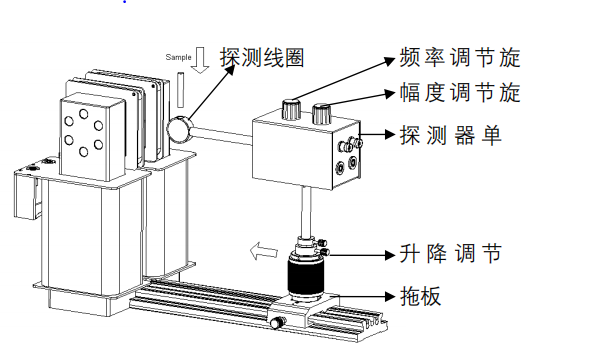
\includegraphics[scale=0.7]{1}
		\end{figure}
		\item 探测单元通过拖板移入磁场中心,旋开高斯计探头的保护套,探头固定在电磁铁顶部的支架上,把探头置于磁场中,调节探头与磁场方向垂直。
		\item 打开可调直流电源,调节电源输出从0~3A,记录高斯计磁场读数于\ref{表1},拟合得到电流-磁场关系。
		\item 取下高斯计,小心地将掺有硫酸铜的水样品放入探测线圈中,并轻轻地推动导轨上的拖
		板,使探测线圈和样品大致置于磁场的中心。
		\item 打开核磁共振试验仪和示波器设备电源开关。设置示波器为CH1通道,电压增益为50或
		100mV,时间增益为2ms。
		\item 调节可调直流电源输出到最左边,即输出为0A。
		\item 调节核磁共振实验仪的扫场幅度调节旋钮到较大幅度(一般为总输出的1/4-1/2,即转
		小半圈左右)。
		\item 调节探测器单元的幅度调节旋钮“AMPLITUDE”到最右边(即顺时针旋到底)。
		\item 调节探测器单元的频率调节旋钮到较小的幅度(即逆时针旋到底后,顺时针旋2圈左右)。
		\item 慢慢地调节直流电源的旋钮,增加电磁铁线圈的电流,加大磁场强度,直到在示波器上
		看到NMR信号,若信号太大或太小,可以调节示波器电压增益旋钮。
		\item 慢慢的调节扫场电源幅度调节旋钮,使共振信号最大(若信号移位或者消失,可以微调
		励磁电流旋钮便可使其出现)。
		\item )慢慢的移动拖板和升降调节架,即改变样品在磁场中的位置,找到共振信号最大最强的
		位置即可(若信号移位或者消失,可以微调励磁电流旋钮便可使其出现)
		\item 调节频率旋钮或者改变励磁电流大小,使共振信号均匀分布(几个信号在示波器x轴上
		等间距)在示波器的显示屏上。
		\item 找到水样品最佳氢核共振信号后,读出核磁共振实验仪表上频率计的显示频率υ,用高 斯计测量磁场的最大值B0,把他们记录在\ref{表2}中。
		\item 通过增加频率υ,重复上述步骤,测量多组数据,计算得到氢核旋磁比。
		\item 更换聚四氟乙烯样品,重复上述步骤(4)-(15),测量多组数据记录在\ref{表3},计算得
		到氟核的旋磁比。
	\end{enumerate}

	
	\begin{table}[H]
		\caption{测量励磁电流-磁场关系曲线}\label{表1}
		\centering
		\begin{tabular}{| c | p{4cm} | p{4cm} |}
		\hline
		 & I(A) & $B_0(mT)$ \\
		\hline
		1 &  &   \\
		\hline
		2 &  &   \\
		\hline
		3 &  &   \\
		\hline
		4 &  &   \\
		\hline
		5 &  &   \\
		\hline
		6 &  &   \\
		\hline
	\end{tabular}
\end{table}
	
	\begin{table}[H]
		\centering
		\caption{测量水样品中氢核旋磁比}
		\label{表2}
	\begin{tabular}{| c | p{4cm} | p{4cm} |}
		\hline
		& $\upsilon(MHz)$ & $B_0(mT)$ \\
		\hline
		1 &  &   \\
		\hline
		2 &  &   \\
		\hline
		3 &  &   \\
		\hline
		4 &  &   \\
		\hline
		5 &  &   \\
		\hline
		6 &  &   \\
		\hline
	\end{tabular}
\end{table}

\begin{table}[H]
	\centering
	\caption{测量聚四氟乙烯样品中氟核旋磁比}\label{表3}
		\begin{tabular}{| c | p{4cm} | p{4cm} |}
		\hline
		& $\upsilon(MHz)$ & $B_0(mT)$ \\
		\hline
		1 &  &   \\
		\hline
		2 &  &   \\
		\hline
		3 &  &   \\
		\hline
		4 &  &   \\
		\hline
		5 &  &   \\
		\hline
		6 &  &   \\
		\hline
	\end{tabular}
\end{table}
	
	\subsubsection{基于已知氢核旋磁比参数,利用核磁共振法精确测量稳恒磁场和扫描磁场大小,并进一步测定磁铁的磁滞回线}
	提示:利用水样品,通过观察氢核的振信号并测量与稳恒磁场强度$B_0$,相对应的共振频率$\upsilon$,利用公式(25)标定磁场强度$B_0$,已知氢核旋磁比$\frac{\gamma}{2\pi}=42.576375 MHz/T$.由于核磁共振实验仪自带频率测量精度(~0.01MHz)不够,可以将射频场信号接入示波器,并通过 USB 接口数据导出,做傅里叶变换得到更高精度频率。同时为了精确测量温恒磁场的大小,逐渐减小扫场幅度$B_m'$至共振信号依然存在,同时调节频率旋钮使共振信号以 10ms 和 20ms 均匀排列,得到共振频率$\upsilon_0=\gamma B_0/2\pi$, $\upsilon_1=\gamma (B_0-B_m')/2\pi$, $\upsilon_2=\gamma (B_0+B_m')/2\pi$.最后
	求得稳恒磁场大小$B_0=(2\upsilon_0+\upsilon_1+\upsilon_2)/(2\gamma /\pi)$和扫描磁场大小$B_m'=\left|\upsilon_1-\upsilon_2\right|/(\gamma/\pi)$将核磁共振法测的$B_0$和高斯计测量结果进行比较.
	
	利用上述精密测量磁场的方法,从小到大,再从大到小改变励磁电流,测出磁体的磁滞回线,作图,并解释同一电流值前后两次测量磁场大小不同的原因。
	\begin{table}[H]
		\centering
		\caption{表4:磁滞回线测量}\label{表4}
		\begin{tabular}{| c | p{4cm} | p{4cm} |}
			\hline
			& $I(mA)$ & $B_0(mT)$ \\
			\hline
			1 &  &   \\
			\hline
			2 &  &   \\
			\hline
			3 &  &   \\
			\hline
			4 &  &   \\
			\hline
			5 &  &   \\
			\hline
			6 &  &   \\
			\hline
			7 &  &   \\
			\hline
			8 &  &   \\
			\hline
		\end{tabular}
	\end{table}
	
	
	\subsubsection{估测固态聚四氟乙烯样品中氟核的驰豫时间}
	提示:示波器改用X-Y输入方式,把“扫场输出”的信号(它与扫场线圈两端并联,电
	压大小相同)输入到X端,“检波输出”信号输入到Y端。调节扫场幅度和共振频率,从示波
	器上观察到的将是重叠而又相互错开了的两个共振峰,如\ref{图11}。利用示波器上的网格估测其
	中一个共振峰的半宽度$\delta B$ 与扫场范围 2B'的比值。然后固定扫场的幅度不变,把示波器改
	回正常的接法,利用实验内容2中方法,求出这时扫场的的峰-峰值2B',进而求出氟核共振
	峰的半宽度$\delta B$,利用公式$$1/T_2=\pi\delta B(\gamma/2\pi)_F$$估算出固态聚四氟乙烯中氟核的驰豫时间。为了更加精确,可以将数据用USB导出,通过洛伦兹线型加上干扰背景信号进行拟合。背景信号可用三阶多项式模拟。
	\begin{figure}[H]
		\centering
		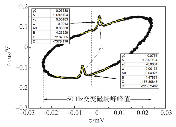
\includegraphics[scale=2]{11}
		\caption{图11 X-Y扫描模式测横向弛豫时间}\label{图11}
	\end{figure}
	
	
	\subsubsection{观察顺磁离子浓度对弛豫时间影响,区分不同水样品(选做)}
	提示:在相同的实验条件下,且满足快通过条件(扫描振幅旋转至>1/2 处),用掺有不
	同浓度顺磁离子的水作样品,观察共振峰的宽度和幅度变化,并利用尾波法估测表观横向弛豫时间,说明顺磁离子浓度对弛豫时间的影响,从而对两管不同水样品进行识别。
	
	尾波法估测表观横向弛豫时间$T_2$:调出不同水样品的氢核共振吸收信号,从示波器中直接读出尾波包络降的数据,如图\ref{图12}所示,利用e指数衰减公式拟合出$T_2$,或者利用示波器USB接口导出尾波信号数据,通过公式数据拟合方式得到$T_2$
	\begin{figure}[H]
		\centering
		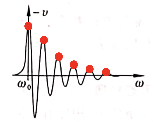
\includegraphics[scale=2]{12}
		\caption{图12 尾波包络降测$T_2$}\label{图12}
	\end{figure}
	
	\subsection{实验过程遇到问题记录}
	
	\subsection{附录:实验数据}




\newpage
\section{分析与讨论}
\begin{tabular}{|p{8em}|p{8em}|p{8em}|p{8em}|}
	\hline 
	专业:     &Physics       &年级:      & 17     \\
	\hline
	姓名:& 徐昊霆 &学号:&17353071  \\
	\hline
	日期&     2019.9               & &  \\
	\hline	
	评分 & & 教师签名 & \\
	\hline
\end{tabular}





\subsection{实验后思考题}


\bibliographystyle{siam}
\bibliography{cites}
\end{document}
